\documentclass[tikz,border=2pt]{standalone}
\usepackage{pgfplots}
\usetikzlibrary{shapes.geometric, intersections}
\pgfplotsset{compat=1.7}

\begin{document}
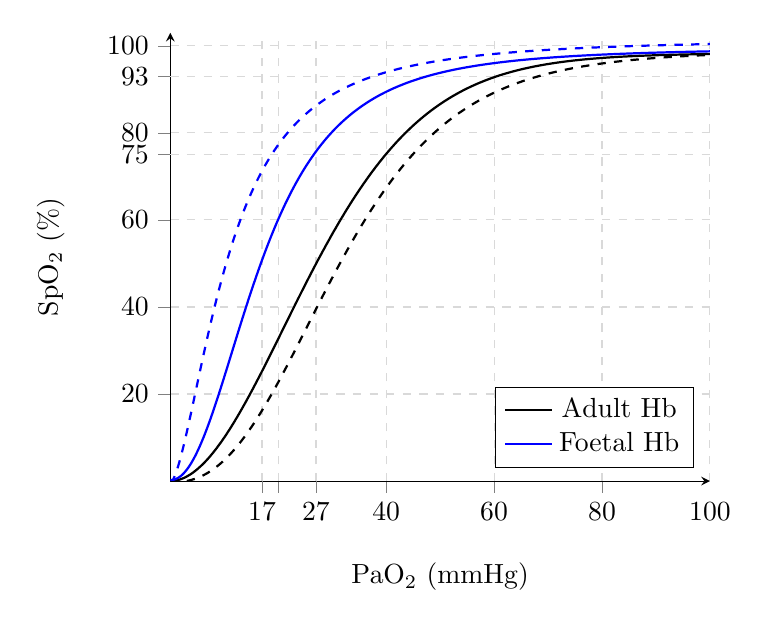
\begin{tikzpicture}

\tikzset{
    myarrow/.style={
        sloped,
        isosceles triangle,
        anchor=apex,
        fill=black,
        inner sep=2pt
    }
}

\makeatletter
\def\parsenode[#1]#2\pgf@nil{%
    \tikzset{label node/.style={#1}}
    \def\nodetext{#2}
}

\tikzset{
    add node at x/.style 2 args={
        name path global=plot line,
        /pgfplots/execute at end plot visualization/.append={
                \begingroup
                \@ifnextchar[{\parsenode}{\parsenode[]}#2\pgf@nil
            \path [name path global = position line #1-1]
                ({axis cs:#1,0}|-{rel axis cs:0,0}) --
                ({axis cs:#1,0}|-{rel axis cs:0,1});
            \path [xshift=1pt, name path global = position line #1-2]
                ({axis cs:#1,0}|-{rel axis cs:0,0}) --
                ({axis cs:#1,0}|-{rel axis cs:0,1});
            \path [
                name intersections={
                    of={plot line and position line #1-1},
                    name=left intersection
                },
                name intersections={
                    of={plot line and position line #1-2},
                    name=right intersection
                },
                label node/.append style={pos=1}
            ] (left intersection-1) -- (right intersection-1)
            node [label node]{\nodetext};
            \endgroup
        }
    },
    add node at y/.style 2 args={
        name path global=plot line,
        /pgfplots/execute at end plot visualization/.append={
                \begingroup
                \@ifnextchar[{\parsenode}{\parsenode[]}#2\pgf@nil
            \path [name path global = position line #1-1]
                ({axis cs:0,#1}-|{rel axis cs:0,0}) --
                ({axis cs:0,#1}-|{rel axis cs:1,1});
            \path [yshift=1pt, name path global = position line #1-2]
                ({axis cs:0,#1}-|{rel axis cs:0,0}) --
                ({axis cs:0,#1}-|{rel axis cs:1,1});
            \path [
                name intersections={
                    of={plot line and position line #1-1},
                    name=left intersection
                },
                name intersections={
                    of={plot line and position line #1-2},
                    name=right intersection
                },
                label node/.append style={pos=1}
            ] (left intersection-1) -- (right intersection-1)
            node [label node] {\nodetext};
            \endgroup
        }
    }
}
\makeatother
    \begin{axis}[
        axis lines=middle,
	ymin = 0,
	ymax = 103,
	xmin = 0,
xmax = 100,
        grid = major,
        grid style={dashed, gray!30},
		extra x ticks={17, 27},
	  xticklabels={,,,40,60,80,100},
	extra x tick labels = {17, 27},
		extra y ticks={75,93},
	extra y tick labels = {75,93},
        xlabel=PaO\textsubscript{2} (mmHg),
        ylabel=SpO\textsubscript{2} (\%),
	 ylabel near ticks,
	xlabel near ticks,
        tick align=outside,
        enlargelimits=false,
legend pos = south east]

	\addplot[domain=0:100, black, thick,samples=500] {98.32157 + (-0.008578349 - 98.32157)/(1 + (x/90.23375)^1.937563)^7.691635};
	\addlegendentry{Adult Hb};
	\addplot[domain=0:100, blue, thick,samples=500] {99.55026 + (0.2308154 - 99.55026)/(1 + (x/21.0583)^2.109015)^1.443303};
	\addlegendentry{Foetal Hb};
	\addplot[domain=0:100, blue, thick, dashed,samples=500] {101.602 + (-0.4369107 - 101.602)/(1 + (x/13.93267)^1.584208)^1.404471};
	\addplot[domain=0:100, black, thick, dashed, samples=500] {98.92857 + (-0.2890872 - 98.92857)/(1 + (x/50.75804)^2.379558)^2.549376};

\end{axis}

\end{tikzpicture} 
\end{document}